% !TEX Root = ../proposal.tex

\section*{}
\subsection*{Motivation}  

\begin{frame} %-----------------------------%
\frametitle{Motivation - Small Satellites} % small satellites
    \begin{itemize}
        \item Spacecraft design/launch and development are costly endeavors
            \begin{itemize}
                \item Long development timelines with extensive component testing
                \item Prohibitive launch costs and manifest scheduling
            \end{itemize}
            \pause
                    
        \begin{tabular}{l | c | c }
            Vehicle & LEO Capacity (\si{\kilogram}) & LEO Cost per \si{\kilogram} \\
            \hline \hline
            Space Shuttle & \num{28803} & \$ \num{10416}  \\ 
            Atlas 2A & \num{8618} & \$ \num{11314} \\
            Falcon 9 & \num{13150} & \$ \num{4654} \\
            Falcon 9 Heavy & \num{53000} & \$ \num{1698}
        \end{tabular}
        
        \item Small spacecraft enable cost effective and rapid development
    
            \begin{itemize}
                \item Reduced size/mass allows for `piggyback' on larger vehicles
                \item Cheaper designs allow for mass production/standardization 
            \end{itemize}

    \end{itemize}
    
    \note[itemize]{
        \item Small sats allow for reduced mass 
        \item Small sats are more responsive and allow more new mission types
    }
\end{frame}   %-----------------------------%

\begin{frame} %-----------------------------%
\frametitle{Motivation - Low Thrust Transfers} % electric propulsion
\begin{itemize}
    \item Low-thrust orbital transfers
    \begin{itemize}
        \item Electric propulsion has increased in popularity

        \includegraphics[height=0.3\textheight]{patriot_plume}
        \hfill
        \includegraphics[height=0.3\textheight]{deepspace1}
 
        \item Offers much higher specific impulse than chemical engines 
        
        \item Requires much longer operating periods for maneuvers 
        \item Small satellites with electric propulsion allows for new mission types
            \begin{itemize}
                \item Formation flight (distributed aperture sensing)
                \item On-orbit servicing
                \item Interplanetary swarms
            \end{itemize}
    \end{itemize}
\end{itemize}
\end{frame}   %-----------------------------%

\begin{frame} %-----------------------------%
\frametitle{Low-thrust vehicles} % electric propulsion
\begin{itemize}
    \item Low-thrust orbital transfers offer increased mission oportunities
    \begin{itemize}
        \item Electric propulsion is increasing in capability
        \item Offers much higher specific impulse than chemical engines 
        \item Requires much longer operating periods for maneuvers 
        \item Enables long duration missions with frequent thrusting
    \end{itemize}
\end{itemize}

\begin{center}
    \includegraphics[width=0.5\textwidth,height=0.5\textheight,keepaspectratio]{figures/patriot_plume.jpg}
    ~
    \includegraphics[width=0.5\textwidth,height=0.5\textheight,keepaspectratio]{figures/deepspace1.jpg}
\end{center}
\end{frame}   %-----------------------------%

\begin{frame}{Asteroids}
\begin{itemize}
    \item Science - insight into the early formation of the solar system
    \item Mining - vast quantities of useful materials
    \item Impact - high risk from hazardous near-Earth asteroids
\end{itemize}    

\begin{center}
    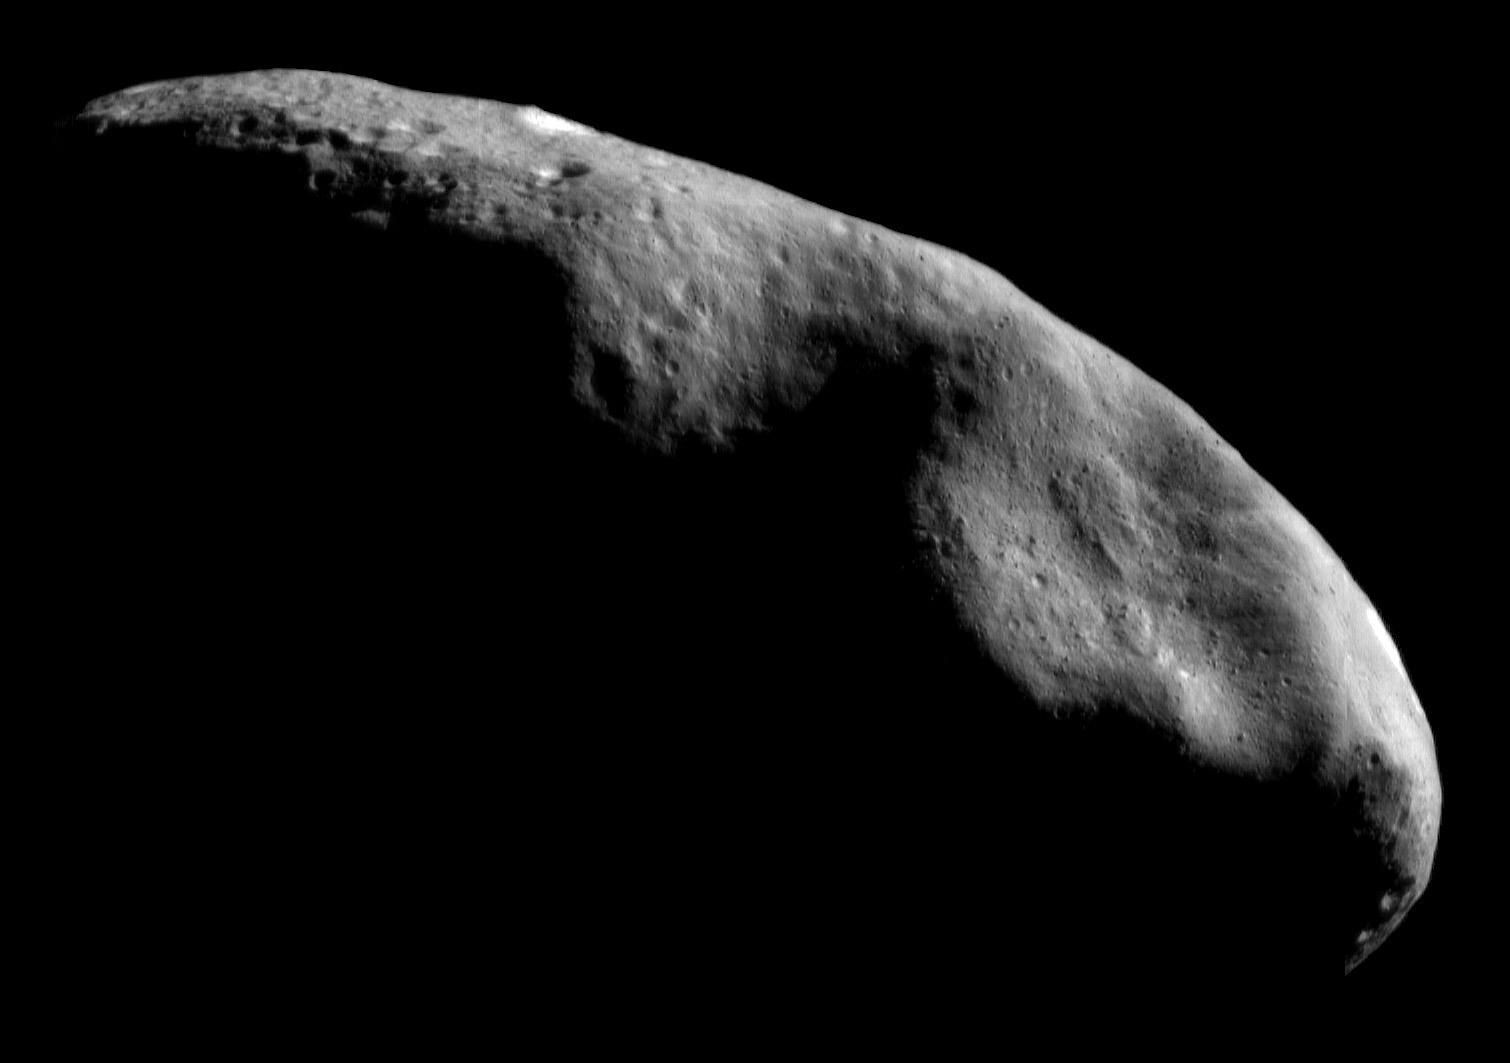
\includegraphics[width=0.5\textwidth,height=0.5\textheight,keepaspectratio]{figures/2016AAS/near_mos_20001203_full.jpg}
    ~
    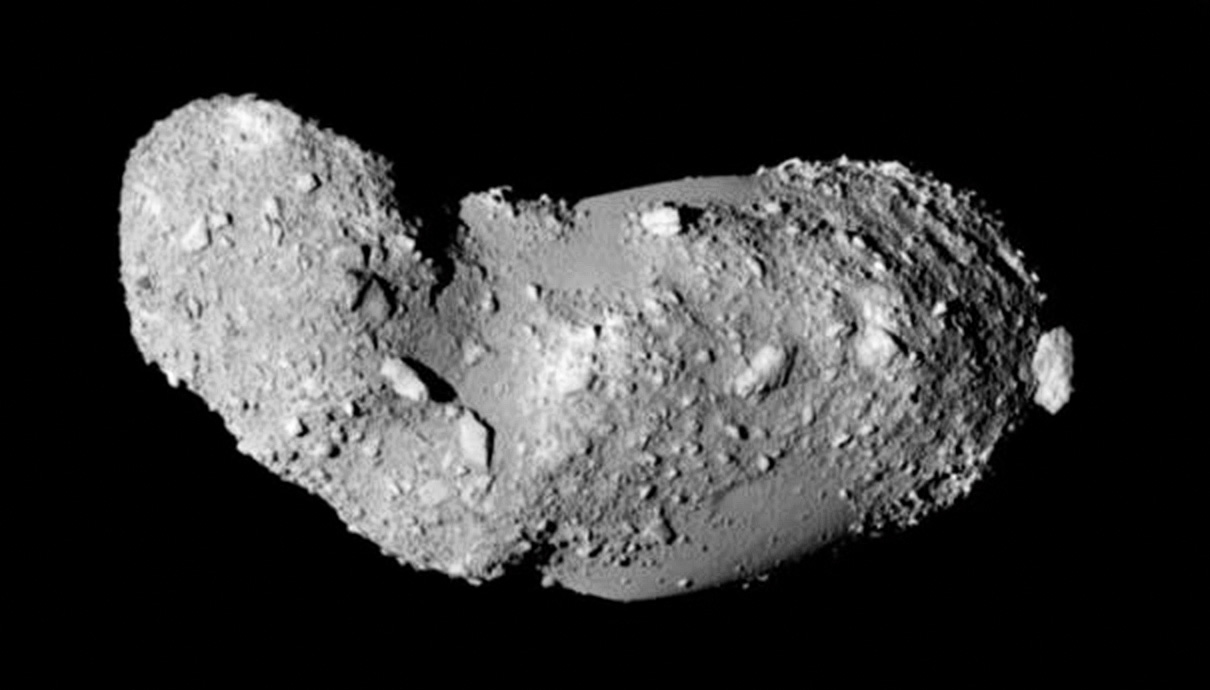
\includegraphics[width=0.5\textwidth,height=0.5\textheight,keepaspectratio]{figures/2016AAS/Itokawa8_hayabusa_1210.jpg}
\end{center}
\end{frame}

\begin{frame}[t]{Motivation} %-----------------------------%
\begin{itemize}
    \item Autonomous control of space vehicles is critical
    \begin{itemize}
        \item Avoid extensive planning and interaction by operators
        \item Ability to operate safely with system uncertainty 
        \item Independently navigate hazards and handle possible failures
    \end{itemize}
\end{itemize}
\visible<2->{
\begin{center}
    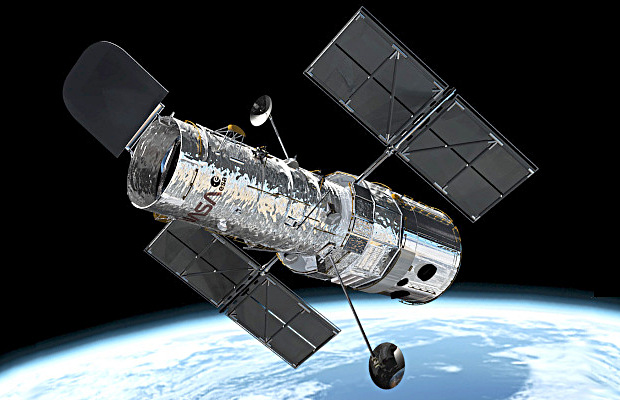
\includegraphics[width=0.5\textwidth,height=0.35\textheight,keepaspectratio]{figures/2016ACC/hubble.jpg}~
    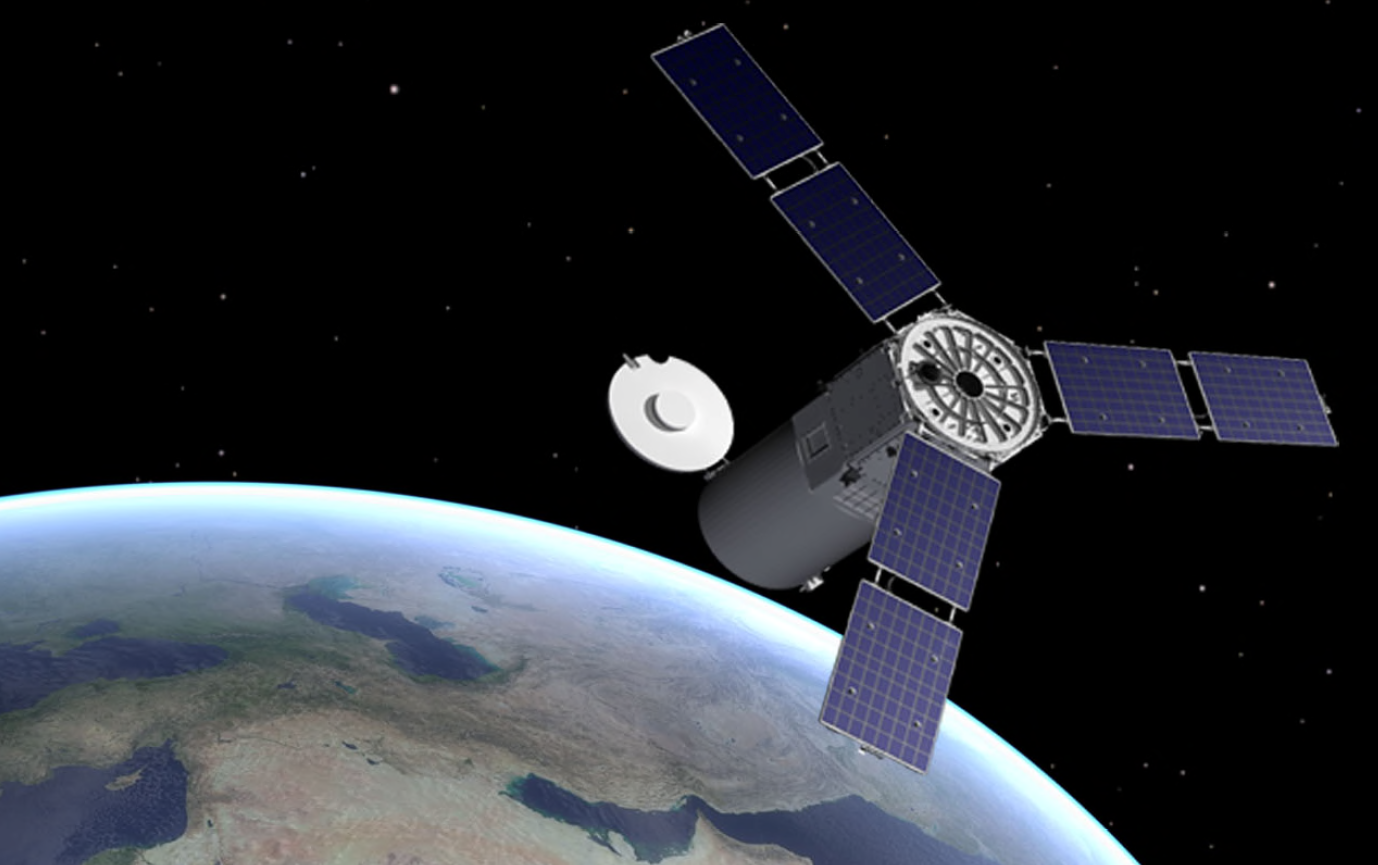
\includegraphics[width=0.5\textwidth,height=0.35\textheight,keepaspectratio]{figures/2016ACC/ors-1.png}
\end{center}
}
\end{frame}   %-----------------------------%